% For an accepted paper, use cameraready and restore author details and acknowledgments.
% The class supports nohyperlinks if requested during final PDF validation.
\documentclass[10pt,doubleanonymous]{ieeeconf}
\usepackage[T1]{fontenc}
\usepackage{float}
\usepackage{amsmath,amssymb,graphicx,booktabs,array,cite,url}
\hypersetup{hidelinks}
\hypersetup{pdftitle={Localized, or Just Lighter? Attributing Background Preservation in Flow-Based Image Editing},pdfauthor={}}
\newcommand{\RMS}{\operatorname{RMS}}
\title{Localized, or Just Lighter? Attributing Background Preservation in Flow-Based Image Editing}

% Generated by analyze_scan.py from the frozen source-level analysis.
% Row schemas and single-point names: scan_macro_contract.md.
\newcommand{\ScanSources}{50}
\newcommand{\ScanPreservationSources}{42}
\newcommand{\ScanSUMean}{0.0326}
\newcommand{\ScanSULo}{0.0204}
\newcommand{\ScanSUHi}{0.0462}
\newcommand{\ScanSUMedian}{0.0199}
\newcommand{\ScanSUWidthMedian}{0.0759}
\newcommand{\ScanSUValid}{41}
\newcommand{\ScanSUEligible}{42}
\newcommand{\ScanSUMissing}{0}
\newcommand{\ScanSUDisjoint}{1}
\newcommand{\ScanSUTouch}{0}
\newcommand{\ScanSUPositive}{37}
\newcommand{\ScanSUZero}{0}
\newcommand{\ScanSUNegative}{4}
\newcommand{\ScanSUNonpositive}{4}
\newcommand{\ScanSFMean}{0.0905}
\newcommand{\ScanSFLo}{0.0625}
\newcommand{\ScanSFHi}{0.1227}
\newcommand{\ScanSFMedian}{0.0532}
\newcommand{\ScanSFWidthMedian}{0.0920}
\newcommand{\ScanSFValid}{38}
\newcommand{\ScanSFEligible}{42}
\newcommand{\ScanSFMissing}{0}
\newcommand{\ScanSFDisjoint}{4}
\newcommand{\ScanSFTouch}{0}
\newcommand{\ScanSFPositive}{35}
\newcommand{\ScanSFZero}{0}
\newcommand{\ScanSFNegative}{3}
\newcommand{\ScanSFNonpositive}{3}
\newcommand{\ScanUFMean}{0.0489}
\newcommand{\ScanUFLo}{0.0220}
\newcommand{\ScanUFHi}{0.0790}
\newcommand{\ScanUFMedian}{0.0274}
\newcommand{\ScanUFWidthMedian}{0.0940}
\newcommand{\ScanUFValid}{41}
\newcommand{\ScanUFEligible}{42}
\newcommand{\ScanUFMissing}{0}
\newcommand{\ScanUFDisjoint}{1}
\newcommand{\ScanUFTouch}{0}
\newcommand{\ScanUFPositive}{32}
\newcommand{\ScanUFZero}{0}
\newcommand{\ScanUFNegative}{9}
\newcommand{\ScanUFNonpositive}{9}
\newcommand{\ScanPairRows}{%
Uniform $-$ SAM native & \ScanSUValid/\ScanSUEligible & \ScanSUMissing/\ScanSUDisjoint/\ScanSUTouch & \ScanSUWidthMedian & \ScanSUMean & [\ScanSULo, \ScanSUHi] & \ScanSUMedian & \ScanSUNonpositive \\
FlowEdit $-$ SAM native & \ScanSFValid/\ScanSFEligible & \ScanSFMissing/\ScanSFDisjoint/\ScanSFTouch & \ScanSFWidthMedian & \ScanSFMean & [\ScanSFLo, \ScanSFHi] & \ScanSFMedian & \ScanSFNonpositive \\
FlowEdit $-$ Uniform & \ScanUFValid/\ScanUFEligible & \ScanUFMissing/\ScanUFDisjoint/\ScanUFTouch & \ScanUFWidthMedian & \ScanUFMean & [\ScanUFLo, \ScanUFHi] & \ScanUFMedian & \ScanUFNonpositive \\}
\newcommand{\ScanPointSOneKnob}{0.25}
\newcommand{\ScanPointSOneResponseN}{50}
\newcommand{\ScanPointSOneResponseMean}{0.0040}
\newcommand{\ScanPointSOneResponseMedian}{0.0061}
\newcommand{\ScanPointSOnePreservationN}{42}
\newcommand{\ScanPointSOnePreservationMean}{0.0091}
\newcommand{\ScanPointSOnePreservationMedian}{0.0063}
\newcommand{\ScanPointSTwoKnob}{0.5}
\newcommand{\ScanPointSTwoResponseN}{50}
\newcommand{\ScanPointSTwoResponseMean}{0.0210}
\newcommand{\ScanPointSTwoResponseMedian}{0.0083}
\newcommand{\ScanPointSTwoPreservationN}{42}
\newcommand{\ScanPointSTwoPreservationMean}{0.0107}
\newcommand{\ScanPointSTwoPreservationMedian}{0.0076}
\newcommand{\ScanPointSThreeKnob}{0.75}
\newcommand{\ScanPointSThreeResponseN}{50}
\newcommand{\ScanPointSThreeResponseMean}{0.0420}
\newcommand{\ScanPointSThreeResponseMedian}{0.0270}
\newcommand{\ScanPointSThreePreservationN}{42}
\newcommand{\ScanPointSThreePreservationMean}{0.0148}
\newcommand{\ScanPointSThreePreservationMedian}{0.0111}
\newcommand{\ScanPointSFourKnob}{1}
\newcommand{\ScanPointSFourResponseN}{50}
\newcommand{\ScanPointSFourResponseMean}{0.0841}
\newcommand{\ScanPointSFourResponseMedian}{0.0585}
\newcommand{\ScanPointSFourPreservationN}{42}
\newcommand{\ScanPointSFourPreservationMean}{0.0297}
\newcommand{\ScanPointSFourPreservationMedian}{0.0240}
\newcommand{\ScanPointSFiveKnob}{1.25}
\newcommand{\ScanPointSFiveResponseN}{50}
\newcommand{\ScanPointSFiveResponseMean}{0.1121}
\newcommand{\ScanPointSFiveResponseMedian}{0.0667}
\newcommand{\ScanPointSFivePreservationN}{42}
\newcommand{\ScanPointSFivePreservationMean}{0.0593}
\newcommand{\ScanPointSFivePreservationMedian}{0.0511}
\newcommand{\ScanPointUOneKnob}{0.25}
\newcommand{\ScanPointUOneResponseN}{50}
\newcommand{\ScanPointUOneResponseMean}{0.0069}
\newcommand{\ScanPointUOneResponseMedian}{0.0058}
\newcommand{\ScanPointUOnePreservationN}{42}
\newcommand{\ScanPointUOnePreservationMean}{0.0101}
\newcommand{\ScanPointUOnePreservationMedian}{0.0076}
\newcommand{\ScanPointUTwoKnob}{0.5}
\newcommand{\ScanPointUTwoResponseN}{50}
\newcommand{\ScanPointUTwoResponseMean}{0.0232}
\newcommand{\ScanPointUTwoResponseMedian}{0.0038}
\newcommand{\ScanPointUTwoPreservationN}{42}
\newcommand{\ScanPointUTwoPreservationMean}{0.0154}
\newcommand{\ScanPointUTwoPreservationMedian}{0.0128}
\newcommand{\ScanPointUThreeKnob}{0.75}
\newcommand{\ScanPointUThreeResponseN}{50}
\newcommand{\ScanPointUThreeResponseMean}{0.0468}
\newcommand{\ScanPointUThreeResponseMedian}{0.0239}
\newcommand{\ScanPointUThreePreservationN}{42}
\newcommand{\ScanPointUThreePreservationMean}{0.0312}
\newcommand{\ScanPointUThreePreservationMedian}{0.0265}
\newcommand{\ScanPointUFourKnob}{1}
\newcommand{\ScanPointUFourResponseN}{50}
\newcommand{\ScanPointUFourResponseMean}{0.0927}
\newcommand{\ScanPointUFourResponseMedian}{0.0639}
\newcommand{\ScanPointUFourPreservationN}{42}
\newcommand{\ScanPointUFourPreservationMean}{0.0947}
\newcommand{\ScanPointUFourPreservationMedian}{0.0737}
\newcommand{\ScanPointUFiveKnob}{1.25}
\newcommand{\ScanPointUFiveResponseN}{50}
\newcommand{\ScanPointUFiveResponseMean}{0.1191}
\newcommand{\ScanPointUFiveResponseMedian}{0.1051}
\newcommand{\ScanPointUFivePreservationN}{42}
\newcommand{\ScanPointUFivePreservationMean}{0.2063}
\newcommand{\ScanPointUFivePreservationMedian}{0.1693}
\newcommand{\ScanPointFOneKnob}{12}
\newcommand{\ScanPointFOneResponseN}{50}
\newcommand{\ScanPointFOneResponseMean}{0.0116}
\newcommand{\ScanPointFOneResponseMedian}{0.0088}
\newcommand{\ScanPointFOnePreservationN}{42}
\newcommand{\ScanPointFOnePreservationMean}{0.0340}
\newcommand{\ScanPointFOnePreservationMedian}{0.0290}
\newcommand{\ScanPointFTwoKnob}{16}
\newcommand{\ScanPointFTwoResponseN}{50}
\newcommand{\ScanPointFTwoResponseMean}{0.0304}
\newcommand{\ScanPointFTwoResponseMedian}{0.0212}
\newcommand{\ScanPointFTwoPreservationN}{42}
\newcommand{\ScanPointFTwoPreservationMean}{0.0478}
\newcommand{\ScanPointFTwoPreservationMedian}{0.0445}
\newcommand{\ScanPointFThreeKnob}{20}
\newcommand{\ScanPointFThreeResponseN}{50}
\newcommand{\ScanPointFThreeResponseMean}{0.0532}
\newcommand{\ScanPointFThreeResponseMedian}{0.0284}
\newcommand{\ScanPointFThreePreservationN}{42}
\newcommand{\ScanPointFThreePreservationMean}{0.0664}
\newcommand{\ScanPointFThreePreservationMedian}{0.0633}
\newcommand{\ScanPointFFourKnob}{24}
\newcommand{\ScanPointFFourResponseN}{50}
\newcommand{\ScanPointFFourResponseMean}{0.0842}
\newcommand{\ScanPointFFourResponseMedian}{0.0712}
\newcommand{\ScanPointFFourPreservationN}{42}
\newcommand{\ScanPointFFourPreservationMean}{0.1185}
\newcommand{\ScanPointFFourPreservationMedian}{0.1091}
\newcommand{\ScanPointFFiveKnob}{28}
\newcommand{\ScanPointFFiveResponseN}{50}
\newcommand{\ScanPointFFiveResponseMean}{0.1446}
\newcommand{\ScanPointFFiveResponseMedian}{0.1684}
\newcommand{\ScanPointFFivePreservationN}{42}
\newcommand{\ScanPointFFivePreservationMean}{0.3546}
\newcommand{\ScanPointFFivePreservationMedian}{0.3608}
\newcommand{\ScanPointRows}{%
SAM native & \ScanPointSOneKnob & \ScanPointSOneResponseN & \ScanPointSOneResponseMean & \ScanPointSOneResponseMedian & \ScanPointSOnePreservationN & \ScanPointSOnePreservationMean \\
SAM native & \ScanPointSTwoKnob & \ScanPointSTwoResponseN & \ScanPointSTwoResponseMean & \ScanPointSTwoResponseMedian & \ScanPointSTwoPreservationN & \ScanPointSTwoPreservationMean \\
SAM native & \ScanPointSThreeKnob & \ScanPointSThreeResponseN & \ScanPointSThreeResponseMean & \ScanPointSThreeResponseMedian & \ScanPointSThreePreservationN & \ScanPointSThreePreservationMean \\
SAM native & \ScanPointSFourKnob$^{*}$ & \ScanPointSFourResponseN & \ScanPointSFourResponseMean & \ScanPointSFourResponseMedian & \ScanPointSFourPreservationN & \ScanPointSFourPreservationMean \\
SAM native & \ScanPointSFiveKnob & \ScanPointSFiveResponseN & \ScanPointSFiveResponseMean & \ScanPointSFiveResponseMedian & \ScanPointSFivePreservationN & \ScanPointSFivePreservationMean \\
Uniform & \ScanPointUOneKnob & \ScanPointUOneResponseN & \ScanPointUOneResponseMean & \ScanPointUOneResponseMedian & \ScanPointUOnePreservationN & \ScanPointUOnePreservationMean \\
Uniform & \ScanPointUTwoKnob & \ScanPointUTwoResponseN & \ScanPointUTwoResponseMean & \ScanPointUTwoResponseMedian & \ScanPointUTwoPreservationN & \ScanPointUTwoPreservationMean \\
Uniform & \ScanPointUThreeKnob & \ScanPointUThreeResponseN & \ScanPointUThreeResponseMean & \ScanPointUThreeResponseMedian & \ScanPointUThreePreservationN & \ScanPointUThreePreservationMean \\
Uniform & \ScanPointUFourKnob$^{*}$ & \ScanPointUFourResponseN & \ScanPointUFourResponseMean & \ScanPointUFourResponseMedian & \ScanPointUFourPreservationN & \ScanPointUFourPreservationMean \\
Uniform & \ScanPointUFiveKnob & \ScanPointUFiveResponseN & \ScanPointUFiveResponseMean & \ScanPointUFiveResponseMedian & \ScanPointUFivePreservationN & \ScanPointUFivePreservationMean \\
FlowEdit & \ScanPointFOneKnob & \ScanPointFOneResponseN & \ScanPointFOneResponseMean & \ScanPointFOneResponseMedian & \ScanPointFOnePreservationN & \ScanPointFOnePreservationMean \\
FlowEdit & \ScanPointFTwoKnob & \ScanPointFTwoResponseN & \ScanPointFTwoResponseMean & \ScanPointFTwoResponseMedian & \ScanPointFTwoPreservationN & \ScanPointFTwoPreservationMean \\
FlowEdit & \ScanPointFThreeKnob & \ScanPointFThreeResponseN & \ScanPointFThreeResponseMean & \ScanPointFThreeResponseMedian & \ScanPointFThreePreservationN & \ScanPointFThreePreservationMean \\
FlowEdit & \ScanPointFFourKnob$^{*}$ & \ScanPointFFourResponseN & \ScanPointFFourResponseMean & \ScanPointFFourResponseMedian & \ScanPointFFourPreservationN & \ScanPointFFourPreservationMean \\
FlowEdit & \ScanPointFFiveKnob & \ScanPointFFiveResponseN & \ScanPointFFiveResponseMean & \ScanPointFFiveResponseMedian & \ScanPointFFivePreservationN & \ScanPointFFivePreservationMean \\}

\makeatletter
\patchcmd{\ieeeconf@printanonymousauthors}{Anonymous submission}{Anonymous ICME Submission.}{}{\ClassError{ieeeconf}{Unexpected anonymous title block}{}}
\makeatother
\begin{document}
\maketitle
\begin{abstract}
A spatial mask changes where an editor acts and how strongly it acts. We separate these effects in two FLUX.1-dev editors. In a source-restoring editor, matching stepwise magnitudes reverses the mean spatial-minus-uniform background LPIPS gap from $+0.0362$ to $-0.0100$. In SAM-Flow, two constants fitted per image recover 84.5\% and 82.4\% of the mean default background gain at seeds 0 and 1, respectively, while reducing directional CLIP on the same 42 images. At default SAM-Flow strength, the edit-to-background MAE ratio is 4.00 for spatial gating at both seeds, compared with 2.11 and 2.03 for uniform gating. Matching directional CLIP within each image over strengths up to default retains 21.3\% and 26.8\% of the default gap on 40 and 41 images with overlapping responses. Matching update magnitude isolates placement at a specified profile. Matching output response compares complete editing configurations.
\end{abstract}

\section{Introduction}
An editor can earn a low background loss on a jar whose lid stays shut. A mask toggle ranks two configurations, but it changes both edit placement and update magnitude. Strength sweeps reveal the preservation--response tradeoff~\cite{meng2022sdedit,brooks2023instruct}.

We compare two FLUX.1-dev editors~\cite{bfl2024flux} across 90 source images (Fig.~\ref{fig:cross}). For a correction toward the source, uniform applies 36.2\% more integrated correction at coefficient 0.25 and gives lower background LPIPS on 39/40 images. Matching stepwise magnitudes reverses the mean ranking. Spatial gives lower loss on 33/40 images at the spatial profile and 31/40 at the uniform profile. SAM-Flow~\cite{cui2026sam} gates displacement away from the source, so even a spatially constant reduction can preserve background.

\begin{figure}[!t]
\centering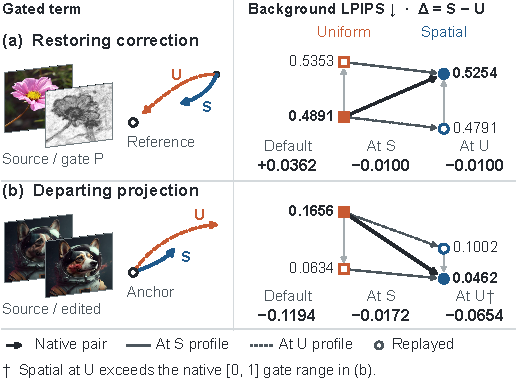
\includegraphics[width=\columnwidth]{figures/v19_cross.pdf}
\caption{\textbf{A mask hides a preservation gain in the restoring editor and enlarges the default gain in SAM-Flow.} Each slope plot uses its own background-LPIPS scale. Default compares the two native configurations. At $S$ and At $U$ compare spatial minus uniform allocation at the same magnitude profile. Negative differences favor spatial allocation. The SAM-Flow panel uses seed 0. At $U$, spatial replay exceeds the native gate range.}
\label{fig:cross}
\end{figure}

DecFlowEdit~\cite{zhan2026decflowedit} compares updates at similar edited-region CLIP and matches guidance norms at a common state. Our crossed profile replay (CPR) applies each native magnitude sequence to both allocations on their own evolving states, yielding a placement contrast at each reference profile.

For configuration choice, matched-response comparison (MRC) compares background loss over the directional-CLIP range both configurations reach on each image. Pixel changes inside and outside the edit region then distinguish a lighter edit from a more localized one.

\begin{figure*}[t]
\centering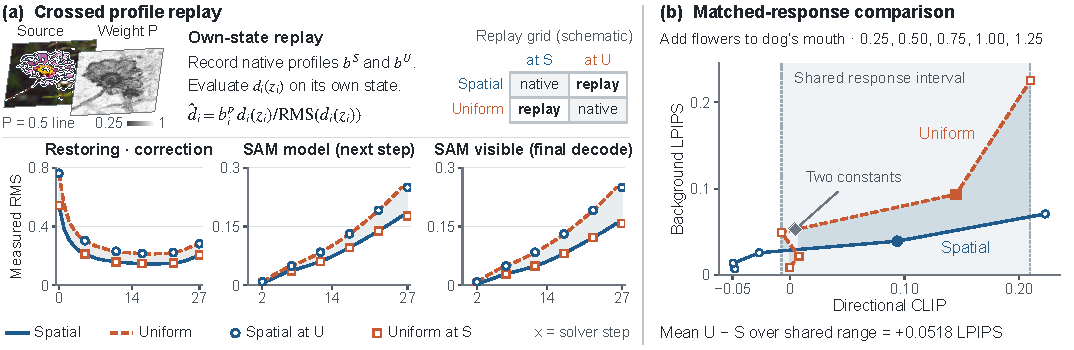
\includegraphics[width=\textwidth]{figures/v19_protocols.pdf}
\caption{\textbf{Replay matches the gated term on the current state.} Uniform applies 44.2\% more integrated correction than spatial on the flower. Across 40 sources the increase is 36.2\% (ratio of means). The two SAM traces and the response curves use the dog in Fig.~\ref{fig:examples}(b). Over its shaded five-setting directional-CLIP range, spatial reduces mean background LPIPS by 0.0518. The diamond denotes the two-constant control.}
\label{fig:protocols}
\end{figure*}

\section{Problem and Protocols}\label{sec:protocol}
\subsection{Magnitude at the intervention site}
Flow models transport samples along a learned velocity field~\cite{lipman2023flowmatching,liu2023rectified}. For a nonzero tensor $v_i$ at step $i$, let $P_{i,j}$ be a weight at spatial location $j$, broadcast over channels $k$. For coefficient $\lambda\ge 0$,
\begin{equation}
\RMS(\lambda P_i\odot v_i)=\lambda\RMS(v_i)
\sqrt{\frac{\sum_{j,k}P_{i,j}^2v_{i,jk}^2}{\sum_{j,k}v_{i,jk}^2}}.
\label{eq:id}
\end{equation}
Weights in $[0,1]$ attenuate the gated term wherever downweighted locations carry energy. The identity holds for any backbone; its consequence for an output ranking depends on the rest of the update, the subsequent trajectory and the decoder~\cite{bradbury2026latentmask}.

Both studies score paired source and edited images at $512\times512$. We compute the spatial AlexNet LPIPS field~\cite{zhang2018lpips} on the full images and average over background pixels. We use this feature-map score (FM) for the main background comparisons. Absolute levels also depend on the source cohort and reconstruction path. Directional CLIP measures the cosine between image and prompt changes~\cite{radford2021clip,gal2022nada} (ViT-L/14 for restoring, ViT-B/32 for SAM). Edit-region MAE measures the size of a pixel change.

\subsection{Crossed profile replay for attribution}
Record both native magnitude profiles $b^S,b^U$. To replay a reference $p$, compute the candidate allocation's direction $d_i$ on its \emph{own} current state $z_i$ and apply
\begin{equation}
   \widehat d_i=b_i^p\,d_i(z_i)/\RMS(d_i(z_i)).
\label{eq:replay}
\end{equation}
A zero target gives a zero update. A positive target requires a nonzero direction. All 100 SAM replays met the FP32 projection tolerance on both branches at every step. After BF16 casting, the sum of absolute errors over 26 steps was at most 0.336\% of the summed target for each source and branch. The worst single-step relative error was 11.39\%. The state-level tolerance ($10^{-6}+0.01b_i$) held at every step on both branches for 3/50 Uniform/$S$ and 34/50 Spatial/$U$ runs. Regional energies, direction, its inner product with the other update terms, and later states can all change. In $L_{a,p}$ the first index denotes allocation and the second the profile donor: Spatial/$U$ uses spatial weights at uniform magnitudes. Two replays per source and seed complete the four cells. Their native loss gap decomposes along either path:

\begin{align}
L_{S,S}-L_{U,U}
&=\underbrace{(L_{S,S}-L_{U,S})}_{\text{allocation at }S}
  +\underbrace{(L_{U,S}-L_{U,U})}_{\text{profile at }U} \nonumber\\
&=\underbrace{(L_{S,U}-L_{U,U})}_{\text{allocation at }U}
  +\underbrace{(L_{S,S}-L_{S,U})}_{\text{profile at }S}.
\label{eq:paths}
\end{align}
Negative allocation contrasts favor spatial. Their difference measures dependence on the reference profile.

\subsection{Matched-response comparison for configuration choice}
For source $s$, sweep the editing control and join adjacent settings in their measured order in the response--loss plane (Fig.~\ref{fig:protocols}). Let $I_s$ be the intersection of the response ranges and $\ell_{a,s}(r)$ the interpolated loss at response $r$. For configurations $U,S$ we estimate
\begin{equation}
D_s=\frac{1}{|I_s|}\int_{I_s}
       [\ell_{U,s}(r)-\ell_{S,s}(r)]\,dr,\qquad
\overline D=\frac{1}{n}\sum_{s\,:\,|I_s|>0}D_s .
\label{eq:mrc}
\end{equation}
For each image with background pixels, we integrate over its positive-width overlap in directional CLIP, then average image estimates with equal weight. Positive $\overline D$ favors spatial allocation. A folded curve uses its first crossing in control order. We also repeat matching at equal edit-region MAE.

\subsection{Relation to prior controls}
Flow editors reuse inverted trajectories~\cite{rout2025rfinversion}, attention or features~\cite{hertz2023prompttoprompt,tumanyan2023pnpfeatures,cao2023masactrl,avrahami2025stableflow}, or source and target velocities~\cite{kulikov2025flowedit,peng2025inversionfree}. A spatial mask can gate denoising~\cite{couairon2023diffedit}, velocity~\cite{li2026veloedit}, or guidance coupled with trajectory injection or step selection~\cite{gong2025instantedit,patel2025flowchef}. Each site calls for a different measurement. Guidance studies distinguish coefficient, direction and active steps~\cite{ho2022cfg,chung2025cfgpp,sadat2025apg,kynkaanniemi2024interval}. GA-Eval calibrates effective guidance; attention-scoped guidance includes a per-sample constant gate~\cite{xie2026guidancematters,li2026asg}. DecFlowEdit's output-level and same-state controls appear in Apps.~D.1 and E.4~\cite{zhan2026decflowedit}. The choice of reference trajectory matters in SAM: the allocation gain is 0.0172 LPIPS at the spatial profile and 0.0654 at the extrapolating uniform profile.

\section{Restoring Correction Hides an Allocation Gain}\label{sec:restoring}
\noindent\textit{Operator and cohort.} On a decreasing schedule let $h_i=\sigma_i-\sigma_{i+1}>0$, let $r_i$ denote the inverted source path, and let $u_i^s$ and $u_i^{t,M_{\rm KV}}$ be the generation-time source and target fields. Only the latter reads the fixed source memory $M_{\rm KV}$. One step is
\begin{align}
c_i(z_i)&=(r_{i+1}-r_i)/h_i-u_i^s(z_i),\nonumber\\
z_{i+1}&=z_i+h_i\{u_i^{t,M_{\rm KV}}(z_i)+\widehat c_i(z_i)\}.
\label{eq:restore}
\end{align}
Native uniform applies $\widehat c_i=0.25c_i$; spatial applies $0.25P\odot c_i$ with $P=1-0.75E$ from three source--target velocity probes. Both share all 28 steps and memory injection, a feature of several flow editors~\cite{wang2025rfsolveredit,deng2025fireflow,zhu2025kvedit}. We average two primary seeds within each of 40 PIE-Bench sources~\cite{ju2024pnpinversion}. Background LPIPS at profile $U$ is the prespecified primary allocation contrast. Intervals resample sources within edit category; the supplement specifies the Holm-adjusted secondary tests.

\noindent\textit{At a shared profile the mean ranking reverses.} At default strength, the mean spatial-minus-uniform background loss is $+0.0362$ [0.0304, 0.0422]. Along both paths a profile term of about $+0.046$ outweighs an allocation term of $-0.010$; at $U$ the latter's 95\% interval is [$-0.0153,-0.0051$]. Spatial changes edit-region pixels more at $U$ (0.1452 versus 0.1367 MAE). At the native settings, edit-to-background MAE ratios are 1.55 for spatial and 1.50 for uniform. The corresponding SAM ratios are farther apart (4.00 and 2.11; Table~\ref{tab:cells}).

\begin{table}[t]
\centering
\caption{Operating points. Lower background (BG) feature-map LPIPS (FM) indicates better preservation. Higher directional CLIP indicates closer alignment of image and text changes. Edit MAE measures change. Higher $S_{\rm MAE}$ indicates greater edit-to-background concentration.}
\label{tab:cells}
{\footnotesize\setlength{\tabcolsep}{1.5pt}
\begin{tabular*}{\columnwidth}{@{\extracolsep{\fill}}lrrrrr@{}}\toprule
 & BG & Dir. & Edit & & \\
Allocation / profile & LPIPS $\downarrow$ & CLIP $\uparrow$ & MAE & $S_{\rm MAE}\!\uparrow$ & $\Delta_a$\\\midrule
\multicolumn{6}{@{}l}{Restoring correction (40 sources, two seeds averaged per source)}\\
Native spatial & 0.5254 & 0.1288 & 0.1646 & 1.55 &\\
Native uniform & 0.4891 & 0.1357 & 0.1367 & 1.50 &\\
One-shot spatial & 0.4853 & 0.1302 & 0.1481 & 1.70 &\\
Uniform / $S$ & 0.5353 & 0.1297 & 0.1587 & 1.42 & $-0.0100$\\
Spatial / $U$ & 0.4791 & 0.1291 & 0.1452 & 1.72 & $-0.0100$\\\midrule
\multicolumn{6}{@{}l}{Departing projection (42 sources with background pixels, seed 0)}\\
Native spatial & 0.0462 & 0.0918 & 0.0628 & 4.00 &\\
Native uniform & 0.1656 & 0.0950 & 0.0869 & 2.11 &\\
Two constants & 0.0646 & 0.0517 & 0.0504 & 2.08 &\\
Uniform / $S^{\dagger}$ & 0.0634 & 0.0553 & 0.0502 & 2.09 & $-0.0172$\\
Spatial / $U^{\dagger}$ & 0.1002 & 0.1198 & 0.1058 & 4.97 & $-0.0654$\\\bottomrule
\end{tabular*}\par
\smallskip\raggedright
All SAM outcome columns use the same 42 sources. $S_{\rm MAE}$ averages the within-image edit/background MAE ratio. The supplement also reports text and edit scores for all 50 sources. At profile $p$, $\Delta_a=L_{S,p}-L_{U,p}$ compares BG LPIPS. Negative values favor spatial allocation.
$^{\dagger}$Uniform/$S$ exceeded the native blend range (coefficient $>1+10^{-6}$) on 2/50 model branches and 0/50 visible branches. Spatial/$U$ exceeded it on both branches for all 50 sources.\par}
\end{table}


\noindent\textit{Calibration and map structure.} A single coefficient fitted per source and seed to the two native integrals yields a spatial-minus-uniform point estimate of $-0.0039$ [$-0.0085,0.0005$]. On its own trajectory it undershoots the target integral by 4.16\% and its loss exceeds stepwise spatial replay at $U$ by 0.0062. Permuting map cells costs 0.0135 LPIPS while changing alignment and smoothness together. A different target prompt yields correlated maps (mean 0.78); the LPIPS contrast spans zero. The organized spatial pattern matters here, while target specificity remains unresolved. The three added seeds, pooled within source, reproduce both matched mean signs; 25/40 images switch individual contrast sign across five seeds.

\noindent\textit{Residual protection inside the edit.} Directional CLIP at $U$ is 0.1291 for spatial and 0.1357 for uniform. The map $P_f=1-(1-f)E$ retains a fraction $f$ of the unweighted correction at maximum probe response before RMS normalization. On 20 sources, removing the 0.25 floor raises directional CLIP by 0.0085 [0.0034, 0.0141]. Against uniform, its CLIP interval spans zero and its mean background loss falls by 0.0137.

\begin{figure*}[t]
\centering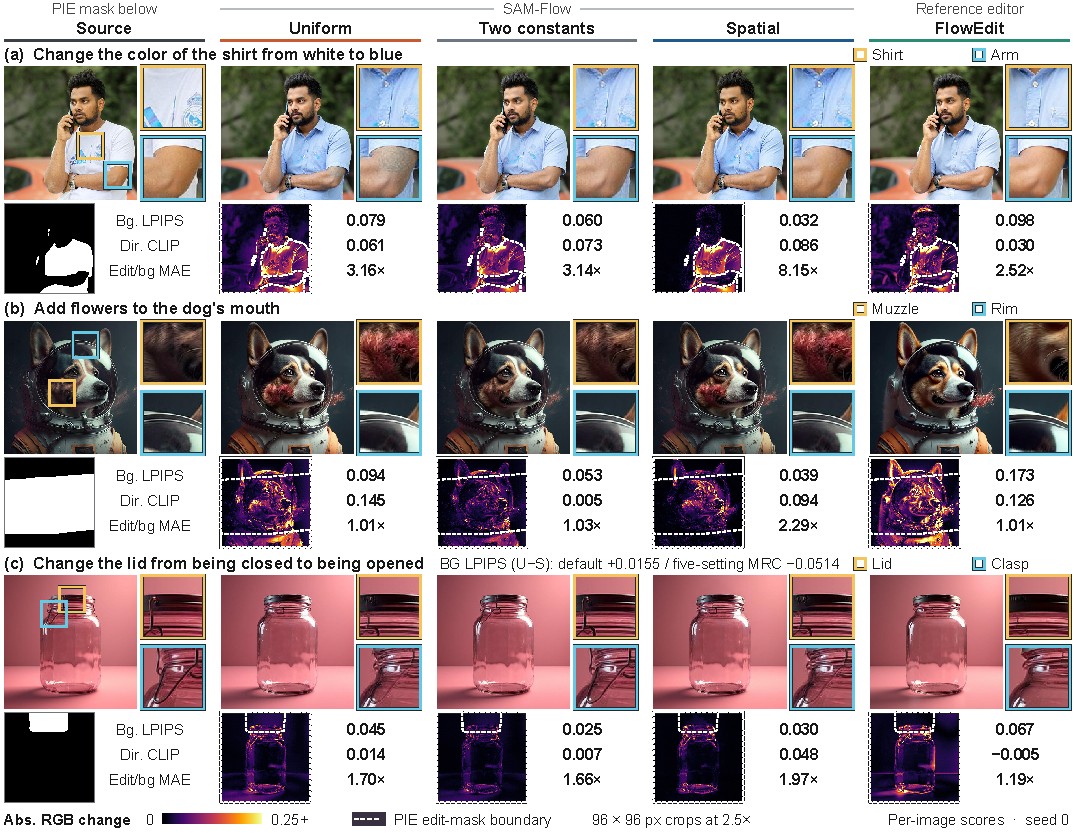
\includegraphics[width=\textwidth]{figures/v19_changes.pdf}
\caption{\textbf{All four outputs show the requested blue shirt in (a); the jar stays closed in (c).} Uniform adds a gray patch below the sleeve. In (b), uniform and spatial add red texture beside the muzzle. The crops show no clearly identifiable flowers in the dog's mouth. The jar favors spatial at default and uniform over the five-setting response overlap. Its four-setting ranges do not overlap. Post hoc examples use aligned $96\times96$ crops ($2.5\times$); dashed outlines mark PIE masks. Heatmaps show mean absolute RGB change, clipped at 0.25 on a shared scale.}
\label{fig:examples}
\end{figure*}

\section{Departing Projection Inflates a Default Gain}\label{sec:depart}
\noindent\textit{Operator and cohort.} Blending with the source can preserve unedited regions~\cite{avrahami2023blendedlatent}. SAM-Flow~\cite{cui2026sam} projects a proposed displacement $R_i$ from source anchor $A$ on two branches. The model state $A+P_i^m\odot R_i$ feeds the next velocity prediction. The visible state $A+P_i^v\odot R_i$ is recomputed at each active step, and the final visible state is decoded. CPR matches each projected displacement's RMS relative to $A$ in FP32 before the state is cast to BF16. The uniform control retains the scout and context processing. The seed-0 study uses 50 PIE-Bench sources (five per category) and 28 steps. At seed 1, all 42 sources with background receive both allocations at four bounded scales, per-image constants and uniform replay at the spatial profile.

\noindent\textit{Spatially constant gains recover much of the default score.} For each image and branch $k$, fit $g_k=\sum_i\RMS(P_i^k\odot R_i)/\sum_i\RMS(R_i)$ on the native spatial trajectory; the new run applies $g_k$ everywhere. The constants retain 84.5\% [78.0\%, 90.5\%] of the default mean background-score gain, measured as $(L_U-L_{\rm const})/(L_U-L_S)$ with cohort means. Their summed magnitude on their own trajectories exceeds the calibration target by 8.42\%. On the same 42 sources, mean directional CLIP falls from 0.0918 to 0.0517 (Table~\ref{tab:cells}). At the constants' response, spatial yields lower background loss on 35/36 supported images (mean difference interval includes zero). To assess transfer across images, we fitted one gain per branch on 49 sources and evaluated the held-out source on its recorded states. Mean visible-branch step error was 18.0\%. At seed 1, per-image constants recover 82.4\% [74.7\%, 89.4\%] of the default background gain as directional CLIP falls from 0.0883 to 0.0461.

\noindent\textit{The reference profile changes the estimated placement gain.} At the spatial profile, spatial minus uniform background LPIPS is $-0.0172$ at seed 0 and $-0.0178$ [$-0.0246$, $-0.0117$] at seed 1. Uniform replay exceeds the blend ceiling on the model branch for 2/50 images at seed 0. Both branches stay within the ceiling tolerance on all 42 images at seed 1. At the uniform profile (seed 0), spatial replay exceeds the ceiling on both branches for all 50 images (maximum factors 2.05 and 4.74 for model and visible). This extrapolated contrast is $-0.0654$. The difference between allocation contrasts is $+0.0481$ [0.0311, 0.0676]. The respective profile terms are $-0.1022$ and $-0.0541$. From the unrounded cells both paths recover the native gap of $-0.119423$.

\section{Matching Response Retains a Smaller Spatial Gain}\label{sec:scan}
The scan compares 750 operating points (150 reused defaults) across five SAM scales, 0.25--1.25, and five FlowEdit window limits, 12--28~\cite{kulikov2025flowedit}. Scale 1 is the SAM default. At scale 1.25 both arms exceed the convex blend range on all 50 sources. The response axis (directional CLIP), first crossing and source-wise overlap were specified before scoring. We harmonized regional LPIPS across operators and examined the four scales at or below default after scoring.

\begin{figure*}[t]
\centering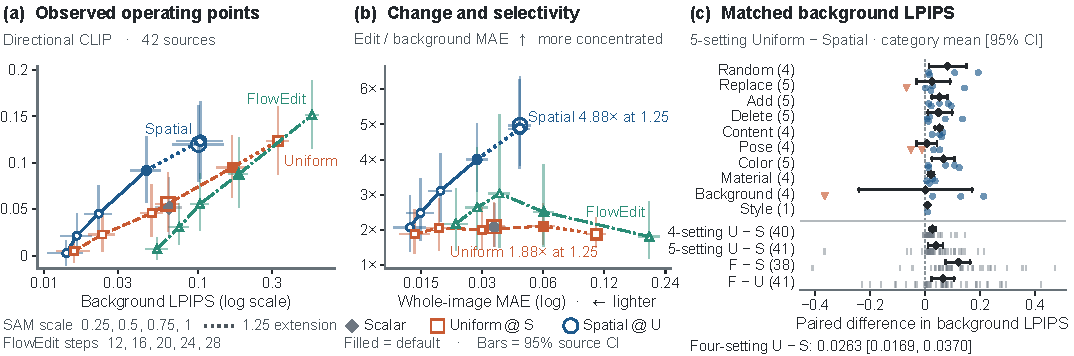
\includegraphics[width=\textwidth]{figures/v19_selectivity.pdf}
\caption{\textbf{At seed 0 and default strength, SAM spatial selectivity reaches 4.00 versus 2.11 for uniform.} In (a,b), points average 42 sources with background pixels. Equation~\eqref{eq:mrc} averages within-image comparisons. Bars give marginal 95\% source-bootstrap intervals. Dotted SAM segments end in open markers at scale 1.25, beyond the convex blend range. Panel (c) reports the four-setting mean for 40 images. Diamonds mark means. Category rows use the five-setting scan (41 images), with triangles for the four favoring uniform.}
\label{fig:scan}
\end{figure*}

At seed 0 and scales 0.25--1.0, 40 of the 42 images with background pixels have overlapping responses. On these 40 images the default uniform-minus-spatial background gap is 0.1233. Four-setting MRC gives a mean FM gap of 0.0263 [0.0169, 0.0370], positive on 37/40 images. This retains 21.3\% [13.2\%, 30.5\%] of the default gap. Seven of the 40 shared intervals lie entirely at nonpositive directional CLIP. On the remaining 33 images, the mean matched gap is 0.0283 [0.0173, 0.0412], or 26.7\% of their mean default gap (0.1060). Integrating only over positive CLIP gives 0.0290. At seed 1, the matched gap is 0.0341 [0.0210, 0.0489] on 41 images, favoring spatial on 37 and retaining 26.8\% [16.3\%, 40.3\%] of the default gap. Excluding eight wholly nonpositive intervals leaves 33 images with a mean matched gap of 0.0418, or 36.9\% of their mean default gap (0.1133). Of the 40 images with overlap at both seeds, 35 favor spatial at both. The paired seed-1 minus seed-0 difference is $+0.0082$ [$-0.0015$, 0.0204].

At seed 0, extending both arms beyond the native gate range to scale 1.25 gives overlap on 41 images and a matched gap of 0.0390 [0.0106, 0.0632], positive on 37/41. Relative to the default gap of 0.1207 on those images, the five-setting scan retains 32.4\% [7.7\%, 57.4\%]. On the same 40 images the five-setting gap is 0.0413. On each image, restricting the integral to the four-setting interval recovers the four-setting estimate. Five of the 41 shared intervals lie entirely at nonpositive directional CLIP. Integrating over positive scores on the remaining 36 images gives 0.0427 [$-0.0018,0.0781$].

\noindent\textit{Where the pixels change.} Write $\rho=\sum_{p\in M_{\rm edit}}\delta_p/\sum_p\delta_p$, where $\delta_p$ is mean absolute RGB change and $M_{\rm edit}$ is the edit mask. The background receives fraction $1-\rho$ of total change. On the 42 seed-0 SAM images, the constants lower whole-image MAE from 0.0600 to 0.0344 while the edit share stays close (uniform 0.380, constants 0.371). Spatial lowers MAE to 0.0283 and raises the share to 0.480. The constants chiefly reduce the amount of change. Spatial weighting also concentrates it inside the edit mask. In the restoring study at $U$, mean total change is almost identical across allocations while spatial raises the edit share by 0.015 [0.008, 0.023].

Pixel selectivity $S_{\rm MAE}$ is the mean of per-image edit/background MAE ratios. Across uniform settings whole-image change grows nearly eightfold but selectivity stays within 1.88--2.11; the constants give 2.08. Spatial selectivity rises from 2.07 at scale 0.25 to 4.00 at the default and 4.88 at the extended scale. At scale 1.25 the two arms have similar cohort-mean directional CLIP (0.1239, 0.1235) and different background LPIPS (0.1033, 0.3268). Equation~\eqref{eq:mrc} addresses within-image response differences.

With scales up to one, uniform has lower matched background LPIPS for the jumping dog, the square crate made round and the rice field. With all five settings, the exceptions are the jumping dog, the reflection, the jar lid and the rice field. The jar favors spatial at default on both background LPIPS (0.030 versus 0.045) and directional CLIP (0.048 versus 0.014). Its response ranges first overlap when scale 1.25 is included, giving $U-S=-0.0514$ in the five-setting comparison. Across the four supported pose edits in that scan, the mean changes sign with the scorer ($+0.0051$ FM, $-0.0013$ masked input). A changed outline may extend outside the source mask.


Aggregation also changes the question. In the restoring editor, the three-setting curve of cohort means favors uniform by 0.0065 directional CLIP at equal background loss. Within-image matching at equal directional CLIP instead favors spatial by 0.0128 LPIPS over 36/40 images with overlap (median width 0.01286). 

\section{Reporting Spatial Ablations}\label{sec:reporting}
Of 24 purposively sampled editing papers, 15 included a within-method regional comparison. None of the 15 records documents matching the realized norm of the gated term at that comparison site. Four document response alignment or a response curve (Table~\ref{tab:literature}). Each paper received one AI assessment. The supplement identifies the comparison, evidence location and coding decision for each paper.
\begin{table}[H]\centering
\caption{Controls at the regional comparison site (15 papers per row). NR means unreported. Toggle counts follow the sheet-specific definitions in the supplement.}
\label{tab:literature}
{\footnotesize\setlength{\tabcolsep}{2pt}
\begin{tabular*}{\columnwidth}{@{\extracolsep{\fill}}lrrrr@{}}\toprule
Control & Yes & No & NR & Unclear\\\midrule
Match realized gated-term norm & 0 & 10 & 5 & 0\\
Align or sweep output response & 4 & 7 & 4 & 0\\
Fixed-setting toggle & 4 & 3 & 0 & 8\\\bottomrule
\end{tabular*}}
\end{table}

\par\medskip\begin{nolinenumbers}\noindent\begin{minipage}{\columnwidth}\centering
\textbf{Checklist for spatial ablations}\par\smallskip
\begin{tabular}{@{}p{.24\columnwidth}p{.69\columnwidth}@{}}
\toprule
Question & Evidence to report\\\midrule
Attribution & Name the gated tensor and report allocation contrasts at both native profiles.\\
Calibration & Check the realized profile against its target and report both outcomes.\\
Configuration & Name the response axis. Report preservation, per-image overlap and paired differences.\\\bottomrule
\end{tabular}
\end{minipage}\par\end{nolinenumbers}\medskip

In a post hoc DirectEdit check on 20 sources~\cite{yang2026directedit}, local-minus-uniform LPIPS is positive at both profiles (local-profile interval includes zero). The primary editors differ in maps, cohorts and operating ranges. Their rankings are consistent with attenuation acting on different terms. CPR measures the allocation effect within each editor.

\noindent\textit{Interpreting a matched score.} Intervals resample sources within a seed and pair shared sources for the seed contrast. MRC compares background LPIPS at the same directional CLIP score, which measures alignment between the image change and the prompt change. Editing benchmarks also examine target objects~\cite{basu2023editval,ma2024i2ebench,qian2025giebench}, protected regions~\cite{wang2023editbench,kim2025augclip} and the requested change itself~\cite{sheynin2024emuedit,baraldi2025changed,ryu2025human,li2025bpm}. The distinction matters for removal and state changes. All 18 moon-removal outputs retain the moon, and the jar in Fig.~\ref{fig:examples} stays closed.

\section{Conclusion}
Matching either correction profile reversed the restoring editor's mean background ranking. In SAM-Flow, spatial allocation concentrated pixel changes at both seeds. Matching directional CLIP over scales up to one retained 21.3\% of the default background gain at seed 0 and 26.8\% at seed 1. Match update magnitudes to attribute placement effects and compare background loss at shared responses to choose configurations.

\section*{AI Disclosure}
OpenAI Codex assisted with manuscript drafting and language editing throughout, analysis code for Sections~\ref{sec:restoring}--\ref{sec:scan}, and preparation of Figs.~\ref{fig:cross}--\ref{fig:scan}. AI agents coded the literature sample in Section~\ref{sec:reporting}. The authors take responsibility for the work.
\begin{thebibliography}{99}
\bibitem{meng2022sdedit}
C. Meng et al., ``SDEdit: Guided image synthesis and editing with stochastic differential equations,'' in \emph{Proc. ICLR}, 2022.

\bibitem{brooks2023instruct}
T. Brooks, A. Holynski, and A. A. Efros, ``InstructPix2Pix: Learning to follow image editing instructions,'' in \emph{Proc. CVPR}, 2023, pp.~18392--18402.

\bibitem{bfl2024flux}
Black Forest Labs, ``FLUX.1-dev,'' model card, 2024. [Online]. Available: \url{https://huggingface.co/black-forest-labs/FLUX.1-dev}

\bibitem{cui2026sam}
H. Cui, R. Chen, T. Luo, T. Guo, Z. Qin, and J. Wang, 
``SAM-Flow: Source-anchored masked flow for training-free image editing,'' arXiv:2606.06228, 2026.

\bibitem{zhan2026decflowedit}
Z. Zhan, C. Wang, J. Chen, C. Chen, S. Lyu, Z. Zheng, and D. Chen,
``DecFlowEdit: Self-localized flow-based image editing via guidance decoupling,'' arXiv:2609.34237, 2026.

\bibitem{lipman2023flowmatching}
Y. Lipman, R. T. Q. Chen, H. Ben-Hamu, M. Nickel, and M. Le,
``Flow matching for generative modeling,'' in \emph{Proc. ICLR}, 2023.

\bibitem{liu2023rectified}
X. Liu, C. Gong, and Q. Liu,
``Flow straight and fast: Learning to generate and transfer data with rectified flow,'' in \emph{Proc. ICLR}, 2023.

\bibitem{bradbury2026latentmask}
R. Bradbury and D. Zhong, ``Your latent mask is wrong: Pixel-equivalent latent compositing for diffusion models,''
in \emph{Proc. CVPR}, 2026, pp.~18630--18639.

\bibitem{zhang2018lpips}
R. Zhang, P. Isola, A. A. Efros, E. Shechtman, and O. Wang,
``The unreasonable effectiveness of deep features as a perceptual metric,'' in \emph{Proc. CVPR}, 2018, pp.~586--595.

\bibitem{radford2021clip}
A. Radford et al.,
``Learning transferable visual models from natural language supervision,'' in \emph{Proc. ICML}, vol.~139, 2021, pp.~8748--8763.

\bibitem{gal2022nada}
R. Gal, O. Patashnik, H. Maron, A. H. Bermano, G. Chechik, and D. Cohen-Or, ``StyleGAN-NADA: CLIP-guided domain adaptation of image generators,'' \emph{ACM Trans. Graph.}, vol.~41, no.~4, Art.~141, 2022.

\bibitem{rout2025rfinversion}
L. Rout, Y. Chen, N. Ruiz, C. Caramanis, S. Shakkottai, and W.-S. Chu,
``Semantic image inversion and editing using rectified stochastic differential equations,'' in \emph{Proc. ICLR}, 2025.

\bibitem{hertz2023prompttoprompt}
A. Hertz, R. Mokady, J. Tenenbaum, K. Aberman, Y. Pritch, and D. Cohen-Or,
``Prompt-to-Prompt image editing with cross-attention control,'' in \emph{Proc. ICLR}, 2023.

\bibitem{tumanyan2023pnpfeatures}
N. Tumanyan, M. Geyer, S. Bagon, and T. Dekel,
``Plug-and-Play diffusion features for text-driven image-to-image translation,'' in \emph{Proc. CVPR}, 2023, pp.~1921--1930.

\bibitem{cao2023masactrl}
M. Cao, X. Wang, Z. Qi, Y. Shan, X. Qie, and Y. Zheng,
``MasaCtrl: Tuning-free mutual self-attention control for consistent image synthesis and editing,'' in \emph{Proc. ICCV}, 2023, pp.~22560--22570.

\bibitem{avrahami2025stableflow}
O. Avrahami et al.,
``Stable Flow: Vital layers for training-free image editing,'' in \emph{Proc. CVPR}, 2025.

\bibitem{kulikov2025flowedit}
V. Kulikov, M. Kleiner, I. Huberman-Spiegelglas, and T. Michaeli,
``FlowEdit: Inversion-free text-based editing using pre-trained flow models,'' in \emph{Proc. ICCV}, 2025, pp.~19721--19730.

\bibitem{peng2025inversionfree}
Z. Peng, C. Yue, T. Duan, and D. Zhang, ``Inversion-free image editing via rectified flow,''
in \emph{Proc. IEEE ICME}, 2025, doi: 10.1109/ICME59968.2025.11209009.

\bibitem{couairon2023diffedit}
G. Couairon, J. Verbeek, H. Schwenk, and M. Cord,
``DiffEdit: Diffusion-based semantic image editing with mask guidance,'' in \emph{Proc. ICLR}, 2023.

\bibitem{li2026veloedit}
Z. Li, Z. Liu, Y. Xie, S. Wu, H. Lv, and S. Su,
``VeloEdit: Training-free consistent and continuous instruction-based image editing via velocity field decomposition,'' arXiv:2603.13388, 2026.

\bibitem{gong2025instantedit}
Y. Gong, Z. Zhu, and M. Zhang, ``InstantEdit: Text-guided few-step image editing with piecewise rectified flow,''
in \emph{Proc. ICCV}, 2025, pp.~16808--16817.

\bibitem{patel2025flowchef}
M. Patel, S. Wen, D. N. Metaxas, and Y. Yang, ``FlowChef: Steering of rectified flow models for controlled generations,''
in \emph{Proc. ICCV}, 2025, pp.~15308--15318.

\bibitem{ho2022cfg}
J. Ho and T. Salimans,
``Classifier-free diffusion guidance,'' arXiv:2207.12598, 2022.

\bibitem{chung2025cfgpp}
H. Chung, J. Kim, G. Y. Park, H. Nam, and J. C. Ye,
``CFG++: Manifold-constrained classifier free guidance for diffusion models,'' in \emph{Proc. ICLR}, 2025.

\bibitem{sadat2025apg}
S. Sadat, O. Hilliges, and R. Weber,
``Eliminating oversaturation and artifacts of high guidance scales in diffusion models,''
in \emph{Proc. ICLR}, 2025.

\bibitem{kynkaanniemi2024interval}
T. Kynk\"{a}\"{a}nniemi, M. Aittala, T. Karras, S. Laine, T. Aila, and J. Lehtinen,
``Applying guidance in a limited interval improves sample and distribution quality in diffusion models,''
in \emph{Advances in Neural Information Processing Systems}, vol. 37, 2024, pp. 122458--122483.

\bibitem{xie2026guidancematters}
D. Xie et al.,
``Guidance matters: Rethinking the evaluation pitfall for text-to-image generation,'' in \emph{Proc. ICLR}, 2026.

\bibitem{li2026asg}
Z. Li, W. Zhou, H. Amirpour, M. Zou, P. Yang, and J. Xu,
``Attention-scoped guidance: Training-free spatial control for image editing,'' arXiv:2609.37492, 2026.

\bibitem{wang2025rfsolveredit}
J. Wang, J. Pu, Z. Qi, J. Guo, Y. Ma, N. Huang, Y. Chen, X. Li, and Y. Shan, ``Taming rectified flow for inversion and editing,''
in \emph{Proc. ICML}, vol.~267, 2025, pp.~64044--64058.

\bibitem{deng2025fireflow}
Y. Deng, X. He, C. Mei, P. Wang, and F. Tang, ``FireFlow: Fast inversion of rectified flow for image semantic editing,''
in \emph{Proc. ICML}, vol.~267, 2025, pp.~13110--13128.

\bibitem{zhu2025kvedit}
T. Zhu, S. Zhang, J. Shao, and Y. Tang, ``KV-Edit: Training-free image editing for precise background preservation,''
in \emph{Proc. ICCV}, 2025, pp.~16607--16617.

\bibitem{ju2024pnpinversion}
X. Ju, A. Zeng, Y. Bian, S. Liu, and Q. Xu,
``PnP inversion: Boosting diffusion-based editing with 3 lines of code,'' in \emph{Proc. ICLR}, 2024.

\bibitem{avrahami2023blendedlatent}
O. Avrahami, O. Fried, and D. Lischinski, ``Blended latent diffusion,''
\emph{ACM Trans. Graph.}, vol.~42, no.~4, Art.~149, 2023, doi: 10.1145/3592450.

\bibitem{yang2026directedit}
D. Yang and M. Ye,
``DirectEdit: Step-level accurate inversion for flow-based image editing,'' in \emph{Proc. ICML}, vol.~306, 2026, pp.~146750--146765.

\bibitem{basu2023editval}
S. Basu et al.,
``EditVal: Benchmarking diffusion based text-guided image editing methods,'' arXiv:2310.02426, 2023.

\bibitem{ma2024i2ebench}
Y. Ma et al.,
``I$^{2}$EBench: A comprehensive benchmark for instruction-based image editing,'' in \emph{Advances in Neural Information Processing Systems}, vol.~37, 2024.

\bibitem{qian2025giebench}
Y. Qian, J. Lu, T.-J. Fu, X. Wang, C. Chen, Y. Yang, W. Hu, and Z. Gan,
``GIE-Bench: Towards grounded evaluation for text-guided image editing,'' arXiv:2505.11493, 2025.

\bibitem{wang2023editbench}
S. Wang et al.,
``Imagen Editor and EditBench: Advancing and evaluating text-guided image inpainting,'' in \emph{Proc. CVPR}, 2023, pp.~18359--18369.

\bibitem{kim2025augclip}
Y. Kim et al.,
``Preserve or modify? Context-aware evaluation for balancing preservation and modification in text-guided image editing,'' in \emph{Proc. CVPR}, 2025, pp.~23474--23483.

\bibitem{sheynin2024emuedit}
S. Sheynin et al.,
``Emu Edit: Precise image editing via recognition and generation tasks,'' in \emph{Proc. CVPR}, 2024, pp.~8871--8879.

\bibitem{baraldi2025changed}
L. Baraldi et al., ``What changed? Detecting and evaluating instruction-guided image edits with multimodal large language models,'' in \emph{Proc. ICCV}, 2025, pp.~16217--16226.

\bibitem{ryu2025human}
S. Ryu, K. Kim, E. Baek, D. Shin, and J. Lee,
``Towards scalable human-aligned benchmark for text-guided image editing,'' in \emph{Proc. CVPR}, 2025, pp.~18292--18301.

\bibitem{li2025bpm}
Z. Li, Z. Xu, Y. Peng, and Y. Liu, ``Balancing preservation and modification: A region and semantic aware metric for instruction-based image editing,'' arXiv:2506.13827, 2025.

\end{thebibliography}

\end{document}
